\documentclass[]{article}

\usepackage{graphicx}
\usepackage[margin=1.0in]{geometry}

%opening
\title{Emory University at TREC LiveQA}
\author{Denis Savenkov\\Emory University\\dsavenk@emory.edu}
\date{}

\begin{document}

\maketitle

\begin{abstract}
This paper describes a question answering system built by a team from Emory University to participate in LiveQA TREC shared task.
Our system extracts candidates from answers to similar previously posted questions as well as from documents retrieved using web search API.
The candidates are ranked using single model, trained on question-answer (QnA) pairs from Yahoo! Answers WebScope dataset\footnote{https://webscope.sandbox.yahoo.com/catalog.php?datatype=l}.
The features used for ranking contains statistics over the candidate answer text, pairs of terms and their matches between question and answer texts and score from an LSTM neural network model, which is also trained on existing QnA pairs.

\end{abstract}

\section{Introduction}
Over the years of question answering research the focus was mainly around factoid questions, which constitute only a part of user information needs.
Community question answering (CQA) websites such as Yahoo! Answers\footnote{http://answers.yahoo.com/} contain millions of questions and answers posted by real users.
These questions are diverse and except factoid include opinion, advice, polls and many other types of questions. 
LiveQA TREC\footnote{http://trec-liveqa.org/} shared task requires a system to answer questions that have been posted to Yahoo! Answers and haven't been answered yet. 
The goal of the task is very interesting, promising and hopefully will lead to development of new systems moving the state-of-the-art in question answering further.

This was my first attempt to participate in TREC and due to time constraints I was able to implement a simple baseline system, which is based on a learning to rank model, trained on existing collection of QnA pairs.
The machine learning system was trained with the objective to rank the ``best''\footnote{By ``best'' we mean the answer that was selected as the best answer to the given question.} answer higher than answers to retrieved similar questions.
The system doesn't use any additional linguistic or other resources and do not try to classify questions into different types.
The goal was to see how well a general purpose system with simple feature can do on questions of various types.

\section{Approach}

\begin{figure}
	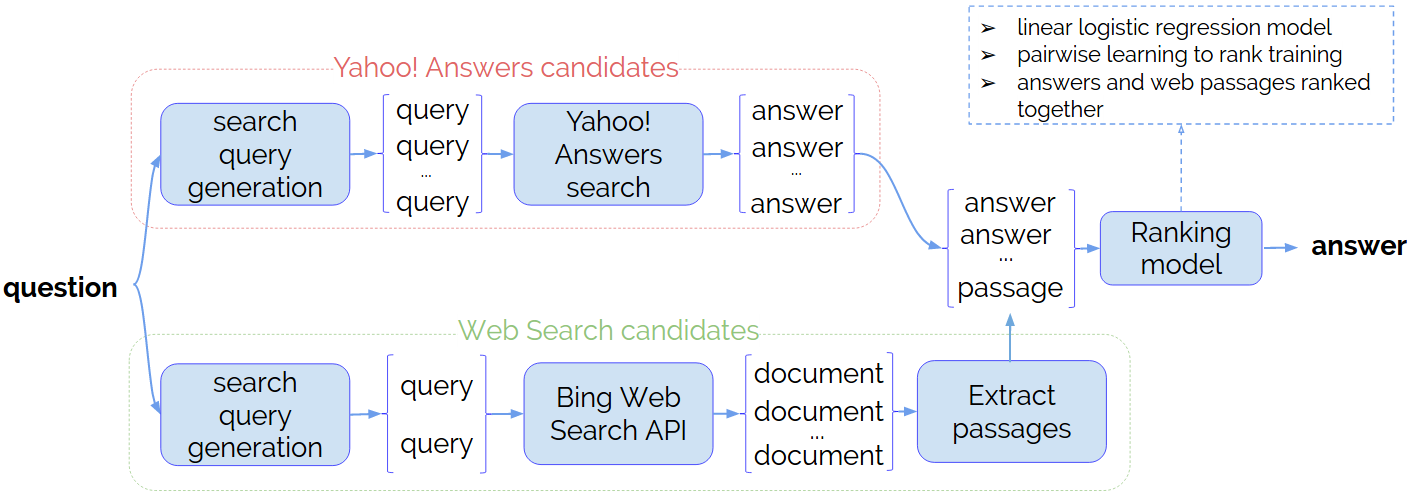
\includegraphics[width=450px]{img/qa_model}
	\caption{Architecture of our question answering system}
	\label{figure:qa_model}
\end{figure}

The general architecture of our question answering system is presented on Figure \ref{figure:qa_model}.
The system uses two primary data sources for generating answer candidates.
People often have similar tasks and situations which generate similar questions, therefore, it's frequently the case that a similar question was already asked by someone and potentially even received a good answer.
Previous research have explored using such data to answer new questions (e.g. \cite{Shtok:2012:LPA:2187836.2187939}), therefore we decided to use answers to previously posted similar questions as the first source of candidates.
However, many questions are still unique and in addition it is often hard to find similar questions in a large collection.
Therefore we also use web search to retrieve some possibly relevant documents and extract candidates from them.
After a set of candidates is generated from both sources, they are combined together in a single pool, features are generated for every one of them and the candidates are ranked with a trained model.
The top candidate is returned as the answer.
Now we will describe all stages in more detail.

\subsection{Candidate generation}
 
Each question issued to a QA system in LiveQA TREC consists of 3 main parts: question title, question body and question category.
For example:

\vspace{0.3cm}
\begin{tabular}{|p{15cm}|}
\hline
\textbf{Question category}: Astronomy \& Space\\
\textbf{Question title}: Why do people claim the Earth isn't the center of the universe?\\
\textbf{Question body}: Clearly the sun and moon are moving around the Earth otherwise we wouldn't have night and day.\\
\hline
\end{tabular}
\vspace{0.3cm}

When our QA system receives a question it first generates a set of candidate answers from Yahoo! Answers and regular web search.
To generate a set of candidates the system produces one or more search queries and issues them to both resources.

To find similar questions and extract the corresponding answers from Yahoo! Answers we use the search functionality already available on the website.
Some questions are very concise while the others provide many useful as well as redundant details.
For many long queries the search doesn't return any results, therefore our system generates a set of search queries of various detail level and issues them all to Yahoo! Answers search and collects top 10 responses from all of them.
Here is the list of queries that our system generates:
For Yahoo! Answers we have many different query formulators:
\begin{itemize}
	\setlength\itemsep{0mm}
	\item Concatenation of question title and question body (with and without stopwords)
	\item Question title only (with and without stopwords)
	\item Question title concatenated with question body and question category
	\item Question title concatenated with the name of the question category
	\item Top 5 terms from question title scored by tf-idf\footnote{Document frequency is computed on WebScope collection of QnA pairs from Yahoo! Answers}
	\item Top 5 terms from question title and body scored by tf-idf
\end{itemize}

For top-10 unique retrieved questions the system extracts the top answer if provided and puts it into the candidate pool along with some information about the corresponding question and its category.

Web search candidate generation is more expensive and we only try two queries for each question: question title and concatenation of title and body.
Recently it was shown \cite{askmsr_plus15} that search engines have improved in processing verbose queries and reformulations are not necessary.
We use Bing Web Search API\footnote{http://datamarket.azure.com/dataset/bing/searchweb} and the system downloads top-10 retrieved documents, parses HTML code and extracts the main content text \cite{Kohlschutter_2010}.
Document content is further split into sentences \cite{manning2014stanford} and candidates are built by taking contiguous sequence of sentences no longer than the answer character limit\footnote{In the final run the limit was 1000 characters}.
We only keep passages that contain at least one non-stopword from the question.

\subsection{Candidate ranking}

To rank the candidate answers we adopt machine learning approach and train a single linear model that scores candidates represented by a set of features (the list of features is given in Table \ref{table:features}).
The candidate with the highest score is returned as the answer to the question.
If something goes wrong and no candidates were generated the system returns ``I don't know'' as the default answer.

\begin{table}[t]
\caption{Features used to rank candidate answers}
\begin{tabular}{|c|p{13cm}|}
\hline
Feature name & Description \\
\hline
\hline
q-a lemma pairs & Concatenation of lemmas from question and answer texts\\
BM25 & BM25 scores of the candidate answer computed for the question title, body and concatenation of both. Collection statistics is taken from WebScope dataset of QnA pairs. \\
term matches & Outputs lemmas of terms matched in the question and answer text as well as percent and the total number of matched terms, POS tags of matched terms, length of the maximum span of matched terms\\
npmi & average, maximum and minimum normalized PMI scores between question and answer terms. NPMI scores are computed based on the WebScope collection of QnA pairs.\\
category match & boolean feature which is one if category of retrieved Yahoo! Answers QnA pair matches one asked\\
page title & Matches between question lemmas and lemmas of the retrieved page title. For Yahoo! Answers question text is used as the title.\\
answer stats & Statistics of the answer text, such as length in sentences in tokens, etc.\\
LSTM model & score returned for QnA pair by an LSTM model trained to predict the correct question-best answer pair\\
\hline
\end{tabular}
\label{table:features}
\end{table}

\subsection{Model Training}

There are two trained models used in the system: LSTM recurrent neural network based model, which is used as one of the features for the final logistic regression model that scores all of the candidate answers.

\subsubsection{LSTM model}

After a huge success of deep learning models in image and speech problems, researchers started to look deeper into applying these techniques to natural language processing and question answering, e.g. \cite{yu2014deep,diwang_lstm_2015}.
We decided to try to build a similar model to produce a score, which can be used as one of the features for the final ranking model.
We chose LSTM recurrent neural network architecture to produce a vector representation of question and answer pair, which is used to make a binary prediction of whether this is a good answer for the question.
Figure \ref{figure:lstm_model} shows a structure of the model.

\begin{figure}
	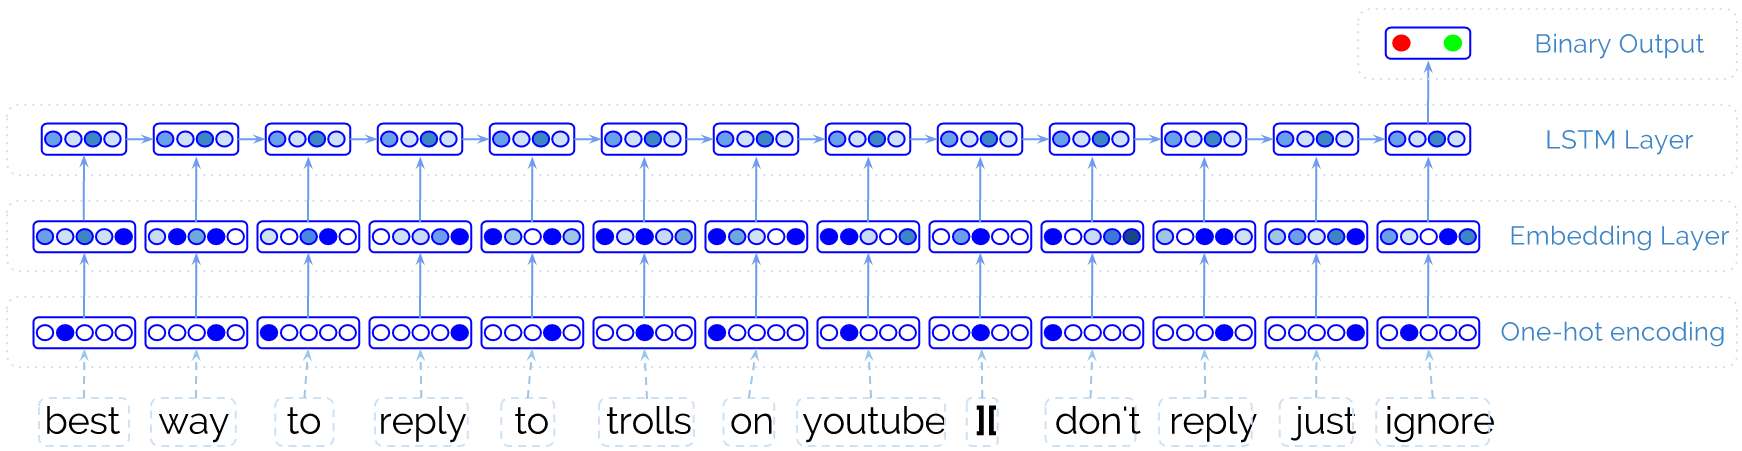
\includegraphics[width=470px]{img/qa_lstm}
	\caption{LSTM model for predicting the correct answer}
	\label{figure:lstm_model}
\end{figure}

Question and answer are tokenized, stopwords and punctuation are removed.
The sequences of tokens are limited to 100 elements and concatenated through a sentinel separator character so the model knew where the question finishes and the answer starts.
The hidden state of the model after it finishes processing a sequence is fed to a logistic unit for a binary class prediction (class 1 represents a good answer for the question and -1 something that doesn't fit well).

To train the model we used a collection of Yahoo! Answers QnA pairs from WebScope dataset.
Each question and the corresponding best answer was used as a positive training example.
To generate negative example we didn't take random example as they will be totally unrelated, and instead we take answers to similar questions.
All questions were indexed with Lucene library and for each question we took answers to 10 other retrieved questions (using BM25 retrieval model) as negative examples.
However, it is true, that a fraction of these answers might as well answer the given question.

The model was implemented using Keras\footnote{http://keras.io} library.
We used an embedding and hidden layers of dimension 128 and the vocabulary size of 1M words (we used hashing to generate word ids).
The model was trained using Adam optimization technique \cite{kingma2014adam} with mini batches of size 200 instances for 100 epochs.

\subsubsection{Logistic regression model}

The final model that ranks all answer candidates is a linear L2-regularized logistic regression model.
To train the model we use a similar setup and also use QnA pairs from Yahoo! Answers WebScope dataset (we use different subsets for training LSTM and logistic regression models). 
For each question and the corresponding correct answer we use Lucene index to retrieve answers to 10 most similar questions.
To train the model we took pairwise approach for learning to rank and generate a training example for pairs of different answers to the same question, where one answer is the correct one.
Each such pair is represented with differences of features of the original answers and an instance is assigned to class 1 if the first answer in the pair is the correct one and to class -1 otherwise.

\section{Results}

Table \ref{table:liveqa-results} gives the results of Emory run and average scores for all runs.

\begin{table}
\caption{Results of the LiveQA evaluation}
\label{table:liveqa-results}
\begin{tabular}{|p{1.2cm}|p{1.2cm}|p{1.2cm}|p{1.2cm}|p{1.2cm}|p{1.2cm}|p{1.2cm}|p{1.2cm}|p{1.2cm}|}
\hline
name & avg score (0-3) & succ@1+ & succ@2+ & succ@3+ & succ@4+ & prec@2+ &
 prec@3+ & prec@4+ \\
 \hline
Emory run & 0.605 & 0.812 & 0.332 & 0.190 & 0.086 & 0.408 & 0.233 & 0.106\\
\hline
Average of all runs & 0.465 & 0.925 & 0.262 & 0.146 & 0.060 & 0.284 & 0.159 & 0.065\\
\hline
\end{tabular}
\end{table}

General statistics:
Overall, 1087 questions were judged and scored using 4-level scale:\\
4: Excellent -- a significant amount of useful information, fully answers the question\\
3: Good – partially answers the question\\
2: Fair -- marginally useful information\\
1: Bad – contains no useful information for the question\\
-2: the answer is unreadable  (only 15 answers from all runs were judged as unreadable)

The performance measures are:\\
avg-score(0-3) - average score over all queries (transferring 1-4 level scores to 0-3, hence comparing 1-level score with no-answer score, also considering -2-level score as 0)\\
succ@i+ - number of questions with i+ score (i=1..4) divided by number of all questions\\
prec@i+ - number of questions with i+ score (i=2..4) divided by number of answered only questions\\

\section{Related Work}

\section{Conclusion}

\bibliographystyle{unsrt}
\bibliography{bibliography.bib}

\end{document}
